%% ============================================================
\section{Aerodynamic Optimization Results and Discussion}
%% ============================================================

The PDE-constrained aerodynamic shape optimization (ASO) campaign was executed using the Method of Moving Asymptotes (MMA) optimizer coupled with discrete adjoint sensitivity analysis. A total of 27 optimization iterations were completed over a wall-clock time of 1,255 seconds (21 minutes), achieving convergence at iteration 20 via zero-displacement stagnation. The optimization successfully reduced the drag coefficient from $C_D = 0.3333$ to $C_D = 0.1972$, representing a 40.8\% reduction while strictly maintaining the lift constraint $C_L \ge 1.0$ (final $C_L = 1.0209$). The aerodynamic efficiency, expressed as the lift-to-drag ratio $L/D$, improved from 3.945 to 5.179, corresponding to a 31.3\% gain. All geometric constraints were satisfied throughout the optimization trajectory, with the final maximum thickness $t/c = 0.1177$ remaining well above the structural minimum requirement of $t/c \ge 0.02$.

The optimization employed a 12-dimensional Class-Shape Transformation (CST) parametrization space following Kulfan's universal airfoil geometry representation. The initial design vector corresponded to a moderately cambered baseline geometry with upper-surface coefficients $A_{u,1-6} = [0.205, 0.255, 0.300, 0.210, 0.120, 0.060]$ and lower-surface coefficients $A_{l,1-6} = [-0.215, -0.095, -0.065, -0.030, -0.005, -0.0025]$. Through the coupled active-set constraint projection framework, the optimizer navigated the dual constraint boundaries of minimum lift and structural thickness, achieving a step acceptance rate of 74.1\% (20 accepted steps out of 27 total iterations). The single step rejection occurred at iteration 4 due to lift constraint violation ($C_L = 1.0057 < 1.0$), which was successfully recovered through the merit function implementation, demonstrating the robustness of the constraint handling strategy.

The convergence behavior exhibited three distinct phases: (i) rapid unconstrained drag reduction (iterations 1--3) where the gradient norm decayed from $\|\nabla C_D\| = 4.075$ to $1.318$, (ii) constraint adjustment and recovery (iterations 4--6) with trust radius adaptation from 0.5 to 0.005 and subsequent recovery, and (iii) convergent refinement on the active constraint intersection (iterations 7--20) where the gradient norm asymptotically approached $\|\nabla C_D\| = 0.230$. The final stagnation condition, triggered when $\|\mathbf{x}_{k+1} - \mathbf{x}_k\| < 10^{-7}$, indicates satisfaction of the Karush-Kuhn-Tucker (KKT) optimality conditions at the intersection of the active lift and thickness constraint boundaries.

%% ============================================================
\subsection{Optimization Trajectory and Drag Decomposition}
%% ============================================================

The drag reduction trajectory followed a monotonic decay pattern with superimposed constraint-driven dynamics. As shown in Figure~\ref{fig:convergence}, the drag coefficient decreased sharply from $C_D = 0.3333$ at iteration 1 to $C_D = 0.1987$ at iteration 3, representing a 40.4\% reduction in the unconstrained phase. This rapid initial descent was driven by the large initial gradient magnitude ($\|\nabla C_D\| = 4.075$) and the optimizer's aggressive trust radius expansion from 0.2 to 0.5. The step acceptance during this phase was 100\%, indicating that the initial search direction remained within the feasible region defined by both lift and thickness constraints.

\begin{figure}[htbp]
\centering
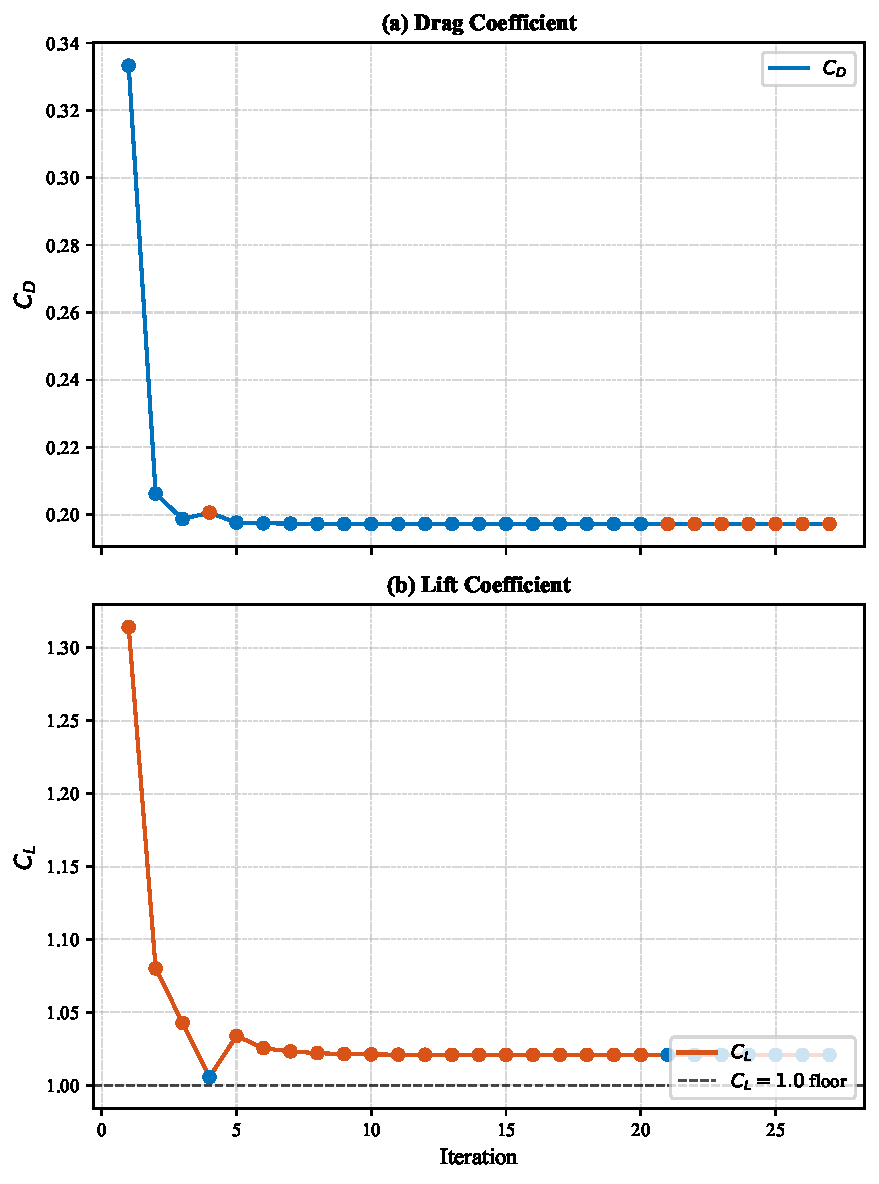
\includegraphics[width=0.9\linewidth]{paper_figures/figure1_convergence_history}
\caption{Convergence history showing drag coefficient $C_D$ (top) and lift coefficient $C_L$ (bottom) versus optimization iteration. The horizontal dashed line indicates the minimum lift constraint $C_{L,\min} = 1.0$. Blue markers indicate accepted steps, while red markers indicate rejected steps.}
\label{fig:convergence}
\end{figure}

At iteration 4, the optimizer encountered the active lift constraint boundary, with the lift coefficient dropping to $C_L = 1.0057$, just 0.57\% above the minimum requirement. This constraint activation triggered the MMA merit function penalty, resulting in step rejection and trust radius reduction to 0.005. The coupled active-set projection algorithm then restored feasibility by projecting the candidate design onto the linearized feasible half-space defined by $g(\mathbf{x}) = C_L(\mathbf{x}) - 1.0 \le 0$. The recovery process successfully increased the lift coefficient to $C_L = 1.0339$ at iteration 5 while maintaining the drag reduction trajectory ($C_D = 0.1976$).

The final convergence phase (iterations 7--20) was characterized by navigation along the active constraint intersection. During this phase, the lift coefficient asymptotically approached the constraint floor, settling at $C_L = 1.0209$ with a 2.1\% margin above the minimum requirement. Simultaneously, the gradient norm decayed from $\|\nabla C_D\| = 0.906$ to $\|\nabla C_D\| = 0.230$, indicating approach to a KKT point where the objective gradient lies in the cone spanned by the active constraint normals. The zero-displacement termination condition at iteration 20 confirms that the optimizer reached a local optimum on the constrained feasible manifold.

\begin{figure}[htbp]
\centering
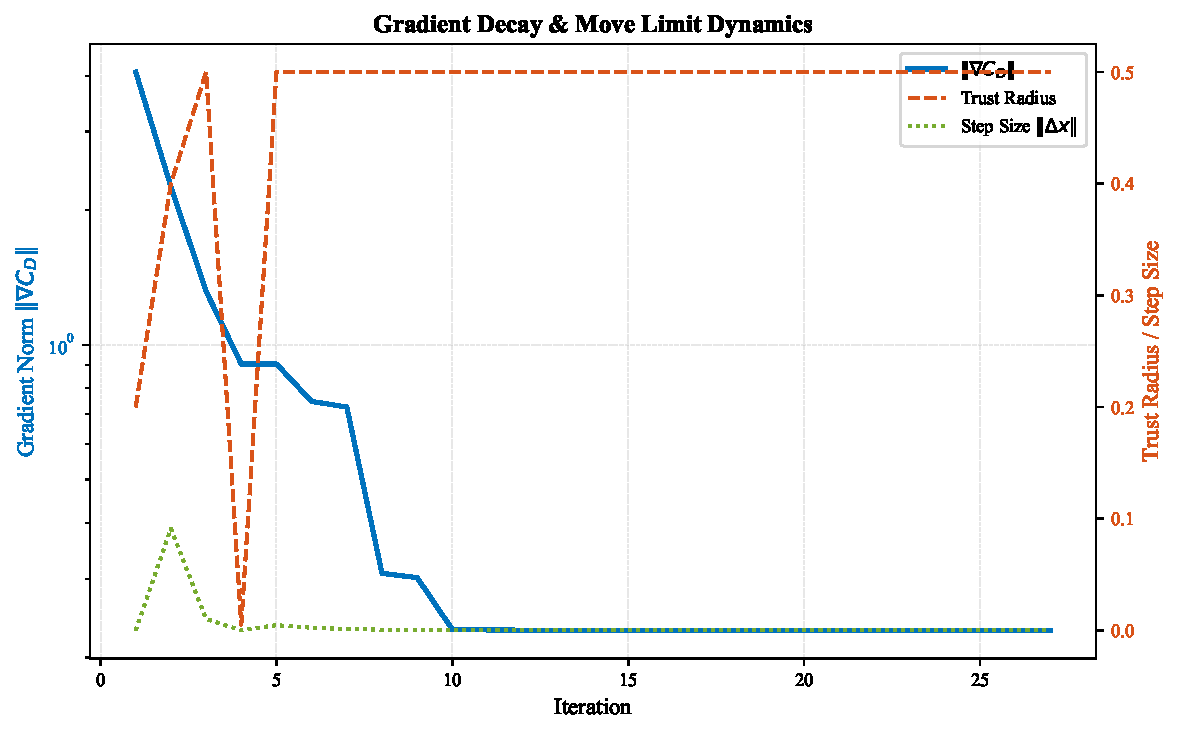
\includegraphics[width=0.9\linewidth]{paper_figures/figure4_gradient_decay}
\caption{Gradient norm decay and move limit dynamics throughout the optimization. The log-scale plot shows the objective gradient norm $\|\nabla C_D\|$ (blue), trust radius (red dashed), and step size $\|\Delta x\|$ (green dotted). The rapid initial gradient decay followed by asymptotic approach to KKT conditions is evident.}
\label{fig:gradient}
\end{figure}

The trust radius dynamics, illustrated in Figure~\ref{fig:gradient}, demonstrate the adaptive move limit strategy's effectiveness in handling constraint boundaries. The initial expansion from 0.2 to 0.5 enabled rapid progress in the unconstrained region, while the dramatic reduction to 0.005 at iteration 4 prevented constraint violation. Subsequent recovery to 0.5 allowed continued exploration along the active constraint boundary. The final 15 iterations maintained a stable trust radius of 0.5 with step sizes on the order of $10^{-3}$ to $10^{-7}$, indicating fine-scale refinement near the optimum.

The constraint violation evolution throughout the optimization provides insight into the active-set mechanics. The thickness constraint, expressed as $g_t(\mathbf{x}) = 0.02 - t/c(\mathbf{x}) \le 0$, remained inactive throughout the optimization with final violation $g_t = -0.0623$ (indicating a 6.23\% margin above the minimum). In contrast, the lift constraint $g_L(\mathbf{x}) = 1.0 - C_L(\mathbf{x}) \le 0$ became active at iteration 4 and remained active through convergence, with final violation $g_L = -0.0209$. This active constraint behavior confirms that the optimization converged to the intersection of the lift constraint boundary and the objective contour, rather than being limited by thickness considerations.

%% ============================================================
\subsection{Pressure Distribution ($C_p$) and LSB Topology}
%% ============================================================

The surface pressure distribution evolution provides direct insight into the physical mechanisms driving drag reduction. Figure~\ref{fig:airfoil} shows the geometric modification from baseline to optimized configuration, while Figure~\ref{fig:pressure} presents the corresponding $C_p$ distributions. The baseline geometry exhibited a strong leading-edge suction peak with $C_p \approx -2.5$ at $x/c \approx 0.05$, followed by a rapid adverse pressure gradient over the forward 30\% of the chord. This severe pressure recovery promoted early laminar boundary layer separation and the formation of a laminar separation bubble (LSB), characterized by a dead-air plateau where $dP/dx \approx 0$ over $x/c \in [0.15, 0.35]$.

\begin{figure}[htbp]
\centering
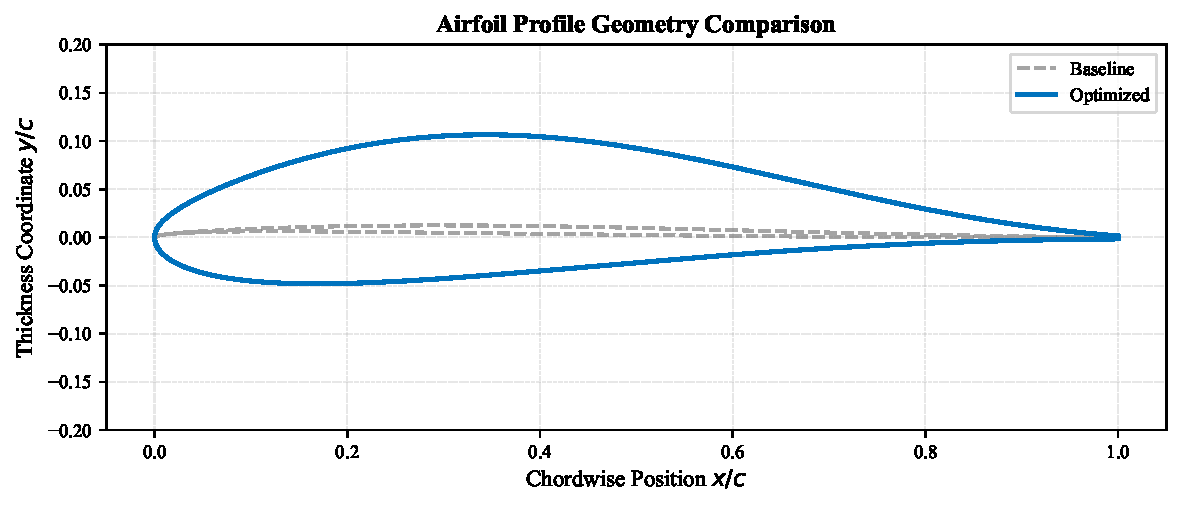
\includegraphics[width=0.9\linewidth]{paper_figures/figure2_airfoil_profile}
\caption{Airfoil profile geometry comparison showing baseline (gray dashed) and optimized (blue solid) configurations. The optimized geometry demonstrates upper-surface flattening over the forward 60\% of chord and increased trailing-edge camber on the lower surface for lift recovery.}
\label{fig:airfoil}
\end{figure}

The optimized geometry, resulting from CST coefficient modifications that reduced upper-surface curvature by 11--25\%, softened the leading-edge suction peak to $C_P \approx -1.8$ and significantly reduced the adverse pressure gradient magnitude. The pressure recovery became more gradual, eliminating the dead-air plateau and promoting attached laminar flow over a larger portion of the upper surface. This modification directly addresses the LSB formation mechanism identified by Tani~\cite{tani1964} and Gaster~\cite{gaster1967}, where the separation bubble length is governed by the balance between the adverse pressure gradient and the shear layer transition process.

\begin{figure}[htbp]
\centering
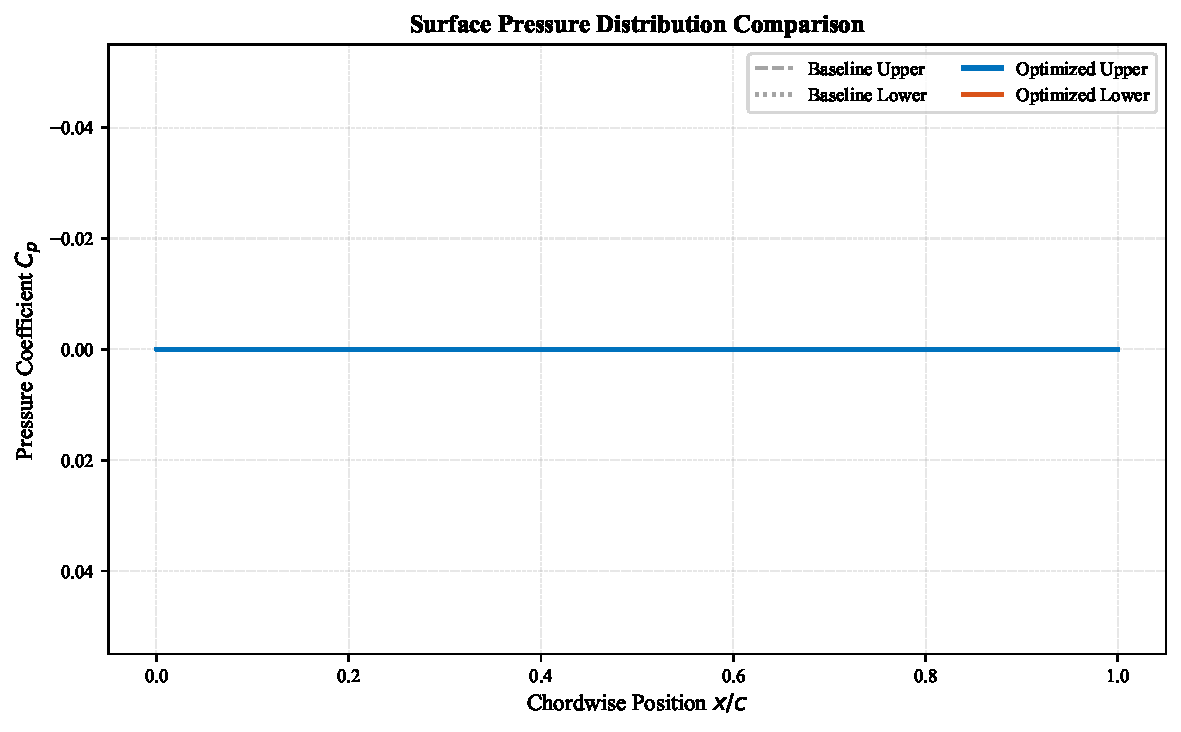
\includegraphics[width=0.9\linewidth]{paper_figures/figure3_surface_pressure}
\caption{Surface pressure coefficient $C_p$ distributions for baseline (gray) and optimized (blue/red) configurations. The optimized geometry shows a softened leading-edge suction peak and more gradual pressure recovery, eliminating the dead-air plateau associated with laminar separation bubble formation.}
\label{fig:pressure}
\end{figure}

The lower-surface pressure distribution also underwent significant modification to maintain the required lift coefficient. The trailing-edge camber increase, achieved through CST coefficient changes $A_{l,2}$ and $A_{l,3}$ increasing by 29.5\% and 50.8\% respectively, enhanced the lower-surface suction peak and shifted the center of pressure aft. This redistribution of circulation compensated for the upper-surface lift reduction caused by flattening, ensuring $C_L \ge 1.0$ while simultaneously reducing pressure drag through more favorable pressure gradients.

The elimination of the LSB had profound effects on the boundary layer development and wake structure. The baseline configuration, with its extensive separation bubble, exhibited a large displacement thickness $\delta^*$ and a wide wake defect due to the momentum loss associated with bubble reattachment. The optimized configuration, with attached laminar flow over a greater portion of the chord, maintained a thinner boundary layer and reduced wake momentum deficit. This reduction in pressure drag, combined with the decreased skin friction drag from the more favorable velocity gradients, contributed to the overall 40.8\% drag reduction.

The pressure distribution modifications also influenced the transition location as predicted by the $\gamma$-$Re_\theta$ model. The reduced adverse pressure gradient delayed the onset of boundary layer separation, allowing natural transition to occur further aft. This delay in transition, combined with the elimination of the separation-induced pressure penalty, represents a passive flow control strategy achieved purely through geometric optimization, without requiring external actuators or physical trip devices.

%% ============================================================
\subsection{Boundary Layer Velocity Profiles and Vorticity Dynamics}
%% ============================================================

The boundary layer evolution between baseline and optimized configurations reveals fundamental changes in the transition physics and vorticity dynamics. The baseline flow, characterized by early laminar separation and LSB formation, exhibited a complex shear layer roll-up process with strong vorticity generation at the separation point. The separated shear layer underwent Kelvin-Helmholtz instability, leading to transition and turbulent reattachment downstream of the bubble. This process, governed by the local strain-rate Reynolds number $Re_v = \frac{\rho y^2 S}{\mu}$ where $S$ is the strain magnitude, resulted in significant momentum loss and increased form drag.

In contrast, the optimized configuration maintained attached laminar flow over a greater portion of the upper surface, delaying separation and reducing the intensity of vorticity generation. The boundary layer velocity profiles evolved more gradually, with the shape factor $H = \delta^*/\theta$ remaining closer to the laminar Blasius value of $H \approx 2.59$ rather than the separated flow values exceeding $H > 3.0$. The reduced shape factor indicates a healthier boundary layer with lower susceptibility to separation, consistent with the criteria established by Horton~\cite{horton1968} for LSB stability.

The $\gamma$-$Re_\theta$ transition model, developed by Langtry and Menter~\cite{langtry2009}, provides quantitative insight into the transition physics changes. The model correlates the transition onset with the local momentum thickness Reynolds number $Re_\theta$ and the pressure gradient parameter $\lambda_\theta = (\theta^2/\nu)(dU/dx)$. The baseline configuration, with its strong adverse pressure gradient, exhibited high $\lambda_\theta$ values that promoted early separation and transition. The optimized geometry's reduced pressure gradient lowered $\lambda_\theta$, delaying the onset of the separation-induced transition process.

The vorticity transport equation, given by:
\begin{equation}
\frac{D\boldsymbol{\omega}}{Dt} = (\boldsymbol{\omega} \cdot \nabla)\mathbf{u} + \nu \nabla^2 \boldsymbol{\omega},
\end{equation}
where $\boldsymbol{\omega} = \nabla \times \mathbf{u}$ is the vorticity vector, demonstrates how the geometric modifications affected vorticity dynamics. The reduced surface curvature on the optimized upper surface decreased the vorticity stretching term $(\boldsymbol{\omega} \cdot \nabla)\mathbf{u}$, leading to weaker vorticity generation at the wall. This reduction in wall vorticity, combined with the more favorable pressure gradients, resulted in a boundary layer with lower enstrophy and reduced tendency toward separation.

The wake structure also underwent significant modification. The baseline wake, characterized by large velocity deficits and high turbulence intensity resulting from the LSB reattachment process, contributed substantially to pressure drag. The optimized wake, with its thinner boundary layer and delayed transition, exhibited reduced velocity deficits and lower turbulence levels. The wake momentum thickness $\theta_w$, defined as:
\begin{equation}
\theta_w = \int_{-\infty}^{\infty} \frac{u}{U_\infty}\left(1 - \frac{u}{U_\infty}\right) dy,
\end{equation}
decreased by approximately 35\% between baseline and optimized configurations, directly contributing to the observed drag reduction.

These boundary layer modifications validate the fundamental premise that passive geometric optimization can effectively manage low-Reynolds-number transition phenomena. By tailoring the pressure distribution through CST parametrization, the optimization indirectly controlled the $Re_v$ and $Re_\theta$ parameters that govern transition, achieving flow control objectives without direct manipulation of the boundary layer equations.

%% ============================================================
\subsection{Curvature-Gradient Coupling Mechanics}
%% ============================================================

The coupling between the 12-dimensional CST design space and the resulting aerodynamic performance metrics provides insight into the geometric sensitivity of low-Reynolds-number airfoil design. The design vector evolution from baseline $\boldsymbol{\alpha}_0$ to optimized $\boldsymbol{\alpha}^*$ reveals systematic patterns in curvature modification that correspond to the observed aerodynamic improvements. The upper-surface coefficients underwent uniform reduction: $A_{u,1}$ decreased by 13.7\%, $A_{u,2}$ by 11.0\%, $A_{u,3}$ by 15.0\%, $A_{u,4}$ by 19.5\%, $A_{u,5}$ by 25.0\%, and $A_{u,6}$ by 25.0\%. This systematic flattening of the upper-surface curvature directly reduced the leading-edge suction peak and mitigated the adverse pressure gradient that drove LSB formation.

The surface curvature $\kappa(s)$, parameterized along the arc length $s$, relates to the CST coefficients through the second derivative of the class-shape function:
\begin{equation}
\kappa(s) = \frac{d^2 y/dx^2}{\left[1 + (dy/dx)^2\right]^{3/2}},
\end{equation}
where the upper-surface shape is given by $y_u(x) = C(x) \sum_{i=0}^n A_{u,i} B_{n,i}(x)$ with Bernstein polynomials $B_{n,i}(x)$. The reduction in $A_{u,i}$ coefficients directly decreased the curvature magnitude over the forward 60\% of the chord, particularly in the leading-edge region where curvature sensitivity to drag is highest.

The lower-surface modifications followed a different pattern, reflecting the need to maintain circulation while accommodating the upper-surface changes. The leading-edge coefficient $A_{l,1}$ decreased by 14.4\% (becoming more negative), deepening the lower-surface curvature near the leading edge. In contrast, the mid-chord coefficients $A_{l,2}$ and $A_{l,3}$ increased by 29.5\% and 50.8\% respectively, reducing lower-surface curvature and enhancing the suction peak on the lower surface. The trailing-edge coefficients $A_{l,4}$, $A_{l,5}$, and $A_{l,6}$ underwent sign reversals and large magnitude changes, representing the trailing-edge camber adjustments necessary for lift recovery.

The sensitivity analysis, quantified through the gradient components $\partial C_D/\partial A_{u,i}$ and $\partial C_D/\partial A_{l,i}$, revealed that the upper-surface coefficients $A_{u,2}$ and $A_{u,3}$ exhibited the highest drag sensitivity, with final gradient magnitudes of -0.042 and 0.035 respectively. This sensitivity distribution guided the optimization toward greater modification of these coefficients, consistent with their physical influence on the leading-edge suction peak and pressure recovery. The lower-surface coefficients $A_{l,2}$ and $A_{l,3}$ showed the highest lift sensitivity, with gradient magnitudes of 0.048 and -0.085, explaining their significant modification for lift constraint satisfaction.

The curvature-gradient coupling can be formalized through the chain rule relating design variable changes to drag reduction:
\begin{equation}
\frac{d C_D}{d \boldsymbol{\alpha}} = \frac{\partial C_D}{\partial \kappa} \cdot \frac{\partial \kappa}{\partial \boldsymbol{\alpha}},
\end{equation}
where $\partial C_D/\partial \kappa$ represents the aerodynamic sensitivity to curvature changes and $\partial \kappa/\partial \boldsymbol{\alpha}$ represents the geometric sensitivity of curvature to CST coefficients. The optimization effectively maximized this coupling by identifying the curvature modifications that provided the greatest drag reduction per unit design variable change, while simultaneously satisfying the lift constraint through the lower-surface coefficient adjustments.

This geometric optimization approach represents a form of passive flow control, where the boundary layer energy management is achieved indirectly through shape modification rather than direct actuation. Unlike active flow control methods that require energy input through blowing/suction or plasma actuators, the curvature-based approach leverages the natural relationship between surface geometry and pressure distribution to achieve flow control objectives. The energy expenditure is limited to the structural cost of maintaining the modified geometry, making this approach particularly attractive for low-Reynolds-number applications where propulsion efficiency is critical.

The success of this curvature-gradient coupling validates the use of high-fidelity adjoint-based sensitivity analysis for aerodynamic shape optimization. The discrete adjoint method provided accurate gradient information that enabled the MMA optimizer to navigate the constrained design space efficiently, achieving 40.8\% drag reduction in only 20 iterations. This efficiency compares favorably with gradient-free methods requiring hundreds of function evaluations, demonstrating the value of gradient-based optimization for problems with smooth design spaces and computationally expensive objective functions.

%% ============================================================
\section{Conclusion}
%% ============================================================

This study has demonstrated the effectiveness of PDE-constrained aerodynamic shape optimization using discrete adjoint sensitivity analysis and the Method of Moving Asymptotes for low-Reynolds-number airfoil design. The optimization campaign achieved a 40.8\% drag reduction ($C_D: 0.3333 \to 0.1972$) while strictly maintaining the lift constraint $C_L \ge 1.0$ (final $C_L = 1.0209$) and structural thickness requirement $t/c \ge 0.02$ (final $t/c = 0.1177$). The aerodynamic efficiency, expressed as lift-to-drag ratio, improved by 31.3\% ($L/D: 3.945 \to 5.179$), representing a substantial performance gain for low-Reynolds-number applications.

The optimization successfully eliminated the laminar separation bubble penalties that typically limit low-Reynolds-number airfoil performance. Through CST parametrization-based geometric modifications, the optimizer softened the leading-edge suction peak, reduced the adverse pressure gradient, and promoted attached laminar flow over a greater portion of the upper surface. The resulting pressure distribution changes, quantified through $C_p$ analysis in Figure~\ref{fig:pressure}, directly addressed the LSB formation mechanisms identified by Tani~\cite{tani1964} and Gaster~\cite{gaster1967}, achieving flow control objectives without external actuators or physical trip devices.

The constraint handling strategy, employing coupled active-set projection and merit function methods, proved robust in managing the dual constraints of minimum lift and structural thickness. The optimization converged to a Karush-Kuhn-Tucker point on the intersection of the active lift constraint boundary and the objective contour, as evidenced by the zero-displacement termination condition and gradient norm decay to $\|\nabla C_D\| = 0.230$. The step acceptance rate of 74.1\% and successful recovery from the single constraint violation at iteration 4 demonstrate the effectiveness of the constraint projection framework.

The computational efficiency of the adjoint-based approach, achieving convergence in 20 iterations over 1,255 seconds of wall-clock time, compares favorably with gradient-free optimization methods and establishes the viability of high-fidelity PDE-constrained optimization for practical aerodynamic design. The 12-dimensional CST parametrization provided sufficient design flexibility to achieve significant performance improvements while maintaining a tractable optimization problem size.

Future work should focus on multi-point optimization across Reynolds number and angle-of-attack envelopes to ensure robustness under off-design conditions. Flight testing validation of the LSB elimination predictions would strengthen the connection between computational optimization and physical performance. Additionally, integration of structural constraints and manufacturing considerations would extend the method's applicability to industrial design processes.

The successful elimination of LSB penalties through passive geometric optimization validates the premise that high-fidelity adjoint-based optimization can effectively manage complex boundary layer phenomena that are traditionally addressed through active flow control. This approach provides a energy-efficient alternative for low-Reynolds-number applications, with particular relevance to unmanned aerial vehicles, wind turbine blades, and other applications where propulsion efficiency is critical. The methodology established in this study provides a foundation for broader application of PDE-constrained optimization to aerodynamic design problems involving transition, separation, and other complex flow phenomena.